\chapter{Kinematics-Based Inter-Arm Distance Monitoring}
\label{chap:distance}

Chapter~\ref{chap:shared_vision} answered \emph{which} arm should act on a jointly visible target,
but the reachability-based role-assignment rule of Equation~\eqref{eq:sv_roleassign} is evaluated
once, at the moment of detection; it says nothing about whether the two arms can move concurrently
in a shared workspace without colliding. Chapter~\ref{chap:lit_review} identified this as gap G3:
conventional collision detection depends either on external sensors or on computationally expensive
algorithms that compromise real-time applicability, and classical geometric formulations provide
only discrete, binary detection rather than the continuous distance metric that modern motion
planners require, while learned detectors are black boxes needing large training
datasets~\citep{sk2025distance,surya2025iapf}.

This chapter presents a kinematics-based framework that closes gap G3. Each manipulator link is
modelled as a line segment in 3D space, positioned directly from forward kinematics and live joint
feedback, so that inter-arm distance is available continuously with no external sensor and no
sensor-to-robot calibration beyond the arms' own kinematic models. Section~\ref{sec:dm_model}
develops the line-segment kinematic model for $N$ arms sharing a workspace.
Section~\ref{sec:dm_classification} classifies the geometric relationship between any two segments
as parallel, intersecting, or skew, and Section~\ref{sec:dm_distance} gives the closed-form
minimum-distance computation for each case. Section~\ref{sec:dm_matrix} assembles these pairwise
distances into a distance matrix restricted to inter-arm segment pairs, and
Section~\ref{sec:dm_dualarm} specializes the general $N$-arm framework to the dual-arm, table-mounted
case that Chapters~\ref{chap:vision_pipelines} and~\ref{chap:shared_vision} have used throughout.
Section~\ref{sec:dm_results} presents real-time hardware validation on dual Kinova Gen3 Lite
manipulators.

%% ============================================================
\section{Line-Segment Kinematic Model}\label{sec:dm_model}
%% ============================================================

Consider $N$ robot manipulators $\{R_1, \ldots, R_N\}$ with joint counts $\{m_1, \ldots, m_N\}$
working in a shared workspace $\mathcal{W} \subset \mathbb{R}^3$. Arm $i$ has joint configuration
$\mathbf{q}_i \in \mathbb{R}^{m_i}$ and its own base frame $B_i$; the aim is to compute the minimum
distance between every pair of links belonging to different arms, in real time, from joint feedback
alone.

Each arm's forward kinematics follows the same chain rule as Equation~\eqref{eq:sv_fwdkin}: for arm
$i$, frame $k$ of its kinematic chain is related to frame $k-1$ by the fixed-geometry, single-DOF
transform $T^{k-1}_{k}(q_i^k)$, and the pose of frame $k$ in the arm's own base frame $B_i$ is the
chained product $T^{B_i}_{k}(\mathbf{q}_i) = T^{B_i}_{1}(q_i^1)\, T^{1}_{2}(q_i^2) \cdots
T^{k-1}_{k}(q_i^k)$. Taking $B_1$ as a shared reference frame, exactly as $B_L$ was taken as the
shared reference in Section~\ref{sec:sv_relay}, and $T^{B_1}_{B_i} \in SE(3)$ as the fixed, calibrated
transform expressing arm $i$'s base frame in that reference (with $T^{B_1}_{B_1} = I$), the position
of joint $k$ of arm $i$ in the shared reference frame is
\begin{equation}
\mathbf{p}_i^k = T^{B_1}_{B_i}\, T^{B_i}_{k}(\mathbf{q}_i)\, \begin{bmatrix} 0 \\ 0 \\ 0 \\ 1 \end{bmatrix}
\in \mathbb{R}^3.
\label{eq:dm_jointpos}
\end{equation}
Each physical link of arm $i$, between consecutive joints $k-1$ and $k$, is modelled as the line
segment
\begin{equation}
L_i^k = \left\{ \mathbf{p}_i^{k-1} + t\left( \mathbf{p}_i^k - \mathbf{p}_i^{k-1} \right) \;\middle|\; t \in [0,1] \right\},
\label{eq:dm_segment}
\end{equation}
and the complete set of link segments across all $N$ arms is
$\mathcal{S} = \{ L_i^k \mid i \in [1,N],\, k \in [1,m_i] \}$.

where ${S}$ is set of all link segments, $L_i^k$ is segment $k$ of arm $i$ and $m_{i}$ is total joints in arm i.

\noindent\textbf{Indexing of the Segment Set:} To address the segments of a heterogeneous multi-arm system, in which the joint counts $m_i$ need not be equal, the total segment count and the cumulative arm offset are defined as
\begin{equation}
M \triangleq |{S}| = \sum_{i=1}^{N} m_i, \qquad
\sigma_i = \sum_{q=1}^{i-1} m_q, \quad \sigma_1 = 0
\label{seg_count}
\end{equation}
The flattening map $\varphi$ and its inverse are then
\begin{equation}
\varphi(i,k) = \sigma_i + k, \qquad i \in [1,N], \; k \in [1,m_i]
\label{phi_map}
\end{equation}
\begin{equation}
i = \max\left\{\, q \in \{1,\ldots,N\} \;\middle|\; \sigma_q < \alpha \,\right\}, \quad k = \alpha - \sigma_i
\label{phi_inv}
\end{equation}
so that $L_\alpha \triangleq L_i^k$ where $(i,k) = \varphi^{-1}(\alpha)$, and the arm-membership function $\rho(\alpha)$ returns the arm index $i$ of segment $\alpha$, satisfying $\rho(\varphi(i,k)) \equiv i$. The map $\varphi$ is a bijection onto $\{1,\ldots,M\}$, and the set in Eq.~\ref{phi_inv} is non-empty for every $\alpha \geq 1$ because $\sigma_1 = 0$, so $\varphi^{-1}$ is defined on the whole index range. For the dual-arm system of Section.~\ref{sec:dm_dualarm}, $\varphi(1,4) = 4$ addresses left arm joint 4 and $\varphi(2,4) = 10$ addresses right arm joint 4.

%% ============================================================
\section{Classification of Link Configurations}\label{sec:dm_classification}
%% ============================================================

For two segments $L_1 = (\mathbf{a}_1, \mathbf{a}_2)$ and $L_2 = (\mathbf{b}_1, \mathbf{b}_2)$, define
direction vectors $\mathbf{u} = \mathbf{a}_2 - \mathbf{a}_1$, $\mathbf{v} = \mathbf{b}_2 - \mathbf{b}_1$,
the vector between start points $\mathbf{w} = \mathbf{b}_1 - \mathbf{a}_1$, and their cross product
$\mathbf{c} = \mathbf{u} \times \mathbf{v}$. Every pair of segments in $\mathbb{R}^3$ falls into
exactly one of three geometric configurations, tested with numerical tolerance
$\varepsilon = 10^{-6}$:
\begin{enumerate}
    \item \textbf{Parallel:} $\lVert \mathbf{c} \rVert < \varepsilon$.
    \item \textbf{Intersecting:} $\lVert \mathbf{c} \rVert \geq \varepsilon$ and
    $\lVert \mathbf{c} \times \mathbf{w} \rVert < \varepsilon$.
    \item \textbf{Skew:} $\lVert \mathbf{c} \rVert \geq \varepsilon$ and
    $\lVert \mathbf{c} \times \mathbf{w} \rVert \geq \varepsilon$.
\end{enumerate}
This classification determines which closed-form distance computation applies, avoiding the
degenerate cases (parallel or intersecting directions) that a single general-purpose formula would
need special-case handling for.

%% ============================================================
\section{Minimum-Distance Computation}\label{sec:dm_distance}
%% ============================================================

The distance function $d : \mathcal{S} \times \mathcal{S} \to \mathbb{R}^{+}$ is non-negative,
$d(L_1, L_2) \geq 0$; symmetric, $d(L_1, L_2) = d(L_2, L_1)$; identical, $d(L, L) = 0$; and continuous
in the segment endpoints. Its closed form depends on the classification of
Section~\ref{sec:dm_classification}.

\textbf{Parallel segments.} The distance reduces to the perpendicular offset between the two
parallel lines, clipped by the segments' finite extent:
\begin{equation}
d_P(L_1, L_2) = \min\left\{ \lVert \operatorname{proj}_{\perp}(\mathbf{w}) \rVert,\; \text{endpoint distances} \right\},
\label{eq:dm_parallel}
\end{equation}
where $\operatorname{proj}_{\perp}(\mathbf{w})$ is the component of $\mathbf{w}$ perpendicular to
both $\mathbf{u}$ and $\mathbf{v}$.

\textbf{Intersecting segments.} Solving the linear system
\begin{equation}
\begin{bmatrix} \mathbf{u} & -\mathbf{v} \end{bmatrix} \begin{bmatrix} s \\ t \end{bmatrix} = \mathbf{w}
\label{eq:dm_intersect}
\end{equation}
for the parameters $s, t$ at which the two infinite lines meet: if the intersection lies on both
segments, $s, t \in [0,1]$, then $d_I(L_1, L_2) = 0$; otherwise the intersection point lies outside
at least one segment and $d_I(L_1, L_2) = \min\{ d(\mathbf{a}_1, L_2),\, d(\mathbf{a}_2, L_2),\,
d(\mathbf{b}_1, L_1),\, d(\mathbf{b}_2, L_1) \}$, the minimum point-to-segment distance over the four
endpoints.

\textbf{Skew segments.} The closest points $\mathbf{p}^* \in L_1$ and $\mathbf{q}^* \in L_2$ satisfy
\begin{equation}
\begin{bmatrix} \mathbf{u}\cdot\mathbf{u} & -\mathbf{u}\cdot\mathbf{v} \\
-\mathbf{u}\cdot\mathbf{v} & \mathbf{v}\cdot\mathbf{v} \end{bmatrix}
\begin{bmatrix} s^* \\ t^* \end{bmatrix} =
\begin{bmatrix} \mathbf{u}\cdot\mathbf{w} \\ -\mathbf{v}\cdot\mathbf{w} \end{bmatrix},
\label{eq:dm_skew}
\end{equation}
and if $s^*, t^* \in [0,1]$, then $d_S(L_1, L_2) = \lVert \mathbf{p}^* - \mathbf{q}^* \rVert$;
otherwise the closest approach of the infinite lines falls outside one or both segments and the
distance is instead computed from the relevant endpoint. This is the case that dominates in
practice: two manipulator links sharing a workspace are generically neither parallel nor
intersecting, so most segment pairs fall here rather than into the two special cases above.

%% ============================================================
\section{The \texorpdfstring{$N$}{N}-Arm Distance Matrix}\label{sec:dm_matrix}
%% ============================================================

The need for a unified representation that captures all inter-arm distances while achieving efficient computation. The distance matrix is,
\begin{equation}
{D} \in \overline{\mathbf{R}}^{\,M \times M}, \quad
D[\alpha,\beta] =
\begin{cases}
d(L_{\alpha}, L_{\beta}), & \rho(\alpha) \neq \rho(\beta)\\
+\infty, & \rho(\alpha) = \rho(\beta)
\end{cases}
\label{dist_matrix}
\end{equation}
where $\overline{\mathbf{R}} = \mathbf{R} \cup \{+\infty\}$. The sentinel value is $+\infty$ rather than zero: since $d(L,L) = 0$ by the identity property, an unevaluated entry initialized to zero would be returned by the global minimum as a spurious collision. The matrix is symmetric, because $d$ is symmetric and the membership test $\rho(\alpha) \neq \rho(\beta)$ is itself symmetric.

\noindent\textbf{Scope:} $D$ is strictly an inter-arm proximity matrix. Intra-arm self-collision is precluded by the joint-limit constraints of the individual manipulator and lies outside the present formulation.

\noindent The elements of ${D[\alpha, \beta]}$ denotes the minimum distance between the segments $\alpha$ and $\beta$ infers proximity database that can be asked for any pair of segments. The distances between intra-arm links are skipped for the computational efficiency, focusing on inter-arm distances as shown in Eq. \ref{eq:dm_intermatrix}.

% Let $\varphi : \{(i,k) \mid i \in [1,N],\, k \in [1,m_i]\} \to \left[1, |\mathcal{S}|\right]$ be a
% fixed bijective index assigning a single linear index to each (arm, link) pair. The unified distance
% matrix is
\begin{equation}
D \in \mathbb{R}^{|\mathcal{S}| \times |\mathcal{S}|}, \qquad D[\varphi(i,k),\, \varphi(l,m)] = d(L_i^k, L_l^m),
\label{eq:dm_fullmatrix}
\end{equation}
% so that $D$ is a proximity database that can be queried for the minimum distance between any two
% segments, from any two arms, without recomputation. Because links belonging to the same arm are
% already governed by that arm's own joint limits and self-collision checks, and because adjacent
% links share a joint and are trivially non-colliding, the distance matrix used for cross-arm
% monitoring is restricted to inter-arm pairs,
\begin{equation}
D\left[ \varphi(i,k),\, \varphi(l,m) \right] \quad \text{where } i \neq l,
\label{eq:dm_intermatrix}
\end{equation}
which is both the physically relevant quantity for inter-arm collision avoidance and, by excluding
same-arm pairs, the computationally cheaper one.

\noindent\textbf{Block Structure:} Grouping the entries of Eq.~\ref{dist_matrix} by arm index yields the inter-arm block
\begin{equation}
D_{il} \in \overline{\mathbf{R}}^{\,m_i \times m_l}, \quad D_{il}[k,m] = d(L_i^{\,k}, L_l^{\,m}), \quad i \neq l
\label{block_eq}
\end{equation}
so that $D$ admits the partition
\begin{equation}
D =
\begin{bmatrix}
\boldsymbol{\infty} & D_{12} & \cdots & D_{1N}\\
D_{12}^{T} & \boldsymbol{\infty} & \cdots & D_{2N}\\
\vdots & \vdots & \ddots & \vdots\\
D_{1N}^{T} & D_{2N}^{T} & \cdots & \boldsymbol{\infty}
\end{bmatrix}
\label{block_partition}
\end{equation}
with $\binom{N}{2}$ populated off-diagonal blocks and $N$ null diagonal blocks. The blocks satisfy $D_{li} = D_{il}^{T}$, since $D_{li}[k, m] = d(L_l^{\,m},L_i^{\,k}) = d(L_i^{\,k},L_l^{\,m}) = D_{il}[k,m]$ by the symmetry of $d$; hence only the pairs $i < k$ need be evaluated. The minimum inter-arm distance of the system follows as
\begin{equation}
d_{\min} = \min_{1 \leq i < k \leq N} \min\left( D_{ik} \right) = \min_{\alpha,\beta} D[\alpha,\beta]
\label{dmin_eq}
\end{equation}
For $N \geq 3$, the individual block minima $\min(D_{ik})$ are available per arm pair in addition to the global minimum of Eq.~\ref{dmin_eq}.

\noindent\textbf{Computational Cost:} Forward kinematics is accumulated incrementally at $O(M)$, and every branch of the distance computation terminates in a bounded number of dot and cross products together with one $2\times2$ solve, so the per-pair cost is $O(1)$. The number of evaluated pairs under the constraint of Eq.~\ref{block_eq}, with the block symmetry exploited, is
\begin{equation}
P = \sum_{1 \leq i < k \leq N} m_i m_k = \frac{1}{2}\left( M^2 - \sum_{i=1}^{N} m_i^2 \right)
\label{pair_count}
\end{equation}
giving a total cost of $O(M^2) = O(N^2 m^2)$ for equal joint counts. For $N = 2$ and $m = 6$ this evaluates to $P = 36$, matching the block size of Eq.~\ref{eq:dm_interarm}. The cost is independent of the configuration, so the method admits a hard worst-case bound, and all $P$ evaluations are mutually independent and therefore parallelizable.


%% ============================================================
\section{Dual-Arm Specialization}\label{sec:dm_dualarm}
%% ============================================================

The general $N$-arm framework above is specialized to the table-mounted dual-arm system used
throughout this thesis: $N = 2$, arms $\mathcal{A}_L$ and $\mathcal{A}_R$ as in
Chapter~\ref{chap:shared_vision}, each with $m_L = m_R = 6$ joints (a Kinova Gen3 Lite), separated
by a fixed base-to-base distance and related by the calibrated inter-arm transform $T^{B_L}_{B_R}$
of Section~\ref{sec:sv_relay} (Figure~\ref{fig:dm_setup}). Table~\ref{tab:dm_dh} lists the
Denavit--Hartenberg parameters used to compute each arm's joint positions via
Equation~\eqref{eq:dm_jointpos}.

\begin{figure}[htbp]
\centering
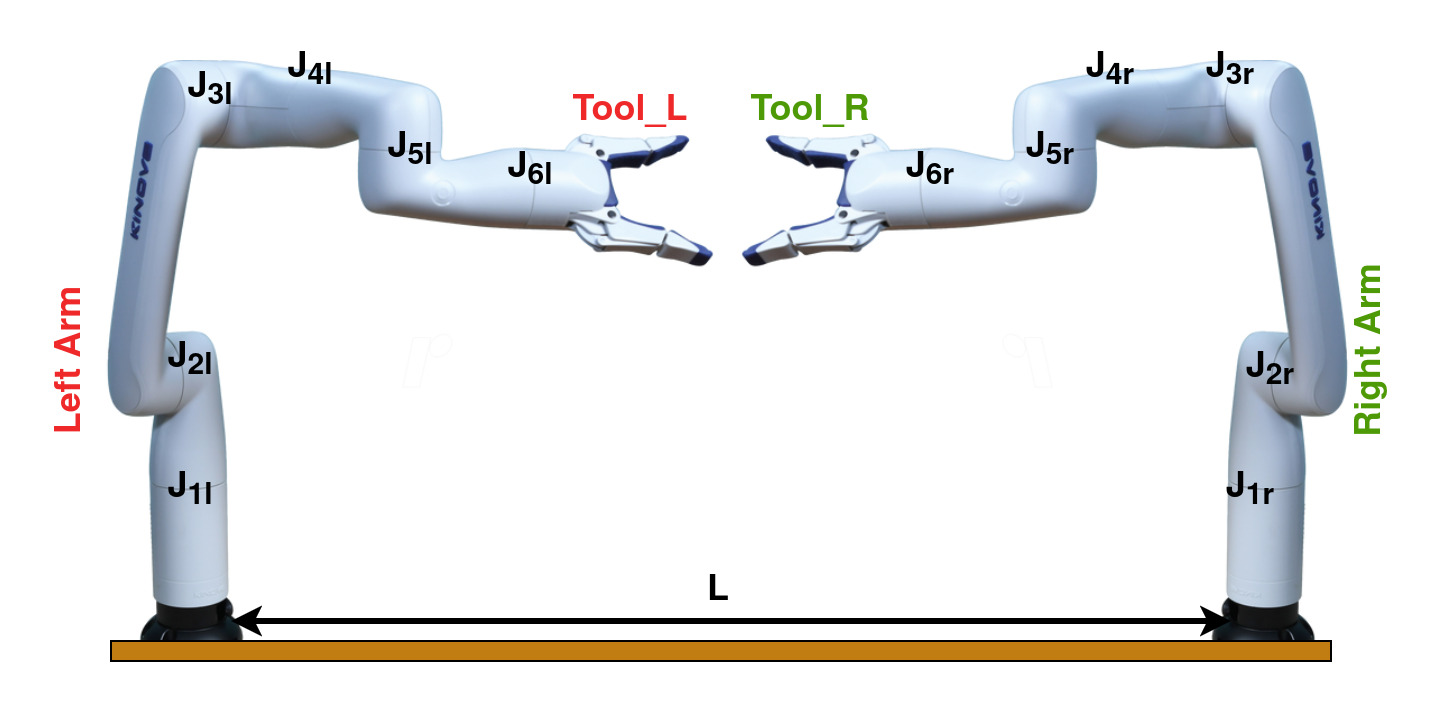
\includegraphics[width=0.75\linewidth]{Images/distanceMonitoring/dual_arm_setup.jpg}
\caption{Dual-arm setup for inter-arm distance calculation~\citep{sk2025distance}.}
\label{fig:dm_setup}
\end{figure}

\begin{table}[htbp]
\centering
\caption{Denavit--Hartenberg parameters for the Kinova Gen3 Lite manipulator, used for line-segment
modelling.}
\label{tab:dm_dh}
\begin{tabular}{ccccc}
\toprule
\textbf{Frame} & $\boldsymbol{\alpha}$ & $\mathbf{a}$ (m) & $\mathbf{d}$ (m) & $\boldsymbol{\theta}$ \\
\midrule
$J_1$ & $\pi/2$ & 0.0   & 0.2433 & $\theta_1$ \\
$J_2$ & $\pi$   & 0.280 & 0.03   & $\theta_2 + \pi/2$ \\
$J_3$ & $\pi/2$ & 0.0   & 0.02   & $\theta_3 + \pi/2$ \\
$J_4$ & $\pi/2$ & 0.0   & 0.245  & $\theta_4 + \pi/2$ \\
$J_5$ & $\pi/2$ & 0.0   & 0.057  & $\theta_5 + \pi$ \\
$J_6$ & 0       & 0.0   & 0.235  & $\theta_6 + \pi/2$ \\
\bottomrule
\end{tabular}
\end{table}

With both arms sharing $B_L$ as the reference frame, the inter-arm distance matrix restricted by
Equation~\eqref{eq:dm_intermatrix} to the six links of each arm is
\begin{equation}
D_{\text{inter}} \in \mathbb{R}^{6 \times 6}, \qquad D_{\text{inter}}[k,m] = d(L_L^k, L_R^m).
\label{eq:dm_interarm}
\end{equation}
In practice, the base separation between the two table-mounted manipulators means the first two
links of each arm, closest to the base, can never approach the other arm closely enough to collide
during normal table operation. Excluding these from the monitored set reduces
Equation~\eqref{eq:dm_interarm} to $D_{\text{inter}} \in \mathbb{R}^{4 \times 4}$, covering links 3
through 6 of each arm, sixteen monitored link pairs in total, without loss of the pairs that can
actually collide.

Algorithm~\ref{alg:dm_collision} summarizes the complete computation, from joint feedback to the
minimum inter-arm distance, executed once per control cycle.

\begin{algorithm}[htbp]
\caption{Multi-Arm Collision Distance Computation}
\label{alg:dm_collision}
\begin{algorithmic}[1]
\REQUIRE Joint configurations $\{\mathbf{q}_1, \mathbf{q}_2, \ldots, \mathbf{q}_N\}$
\ENSURE Minimum distance between any pair of segments from different arms
\FOR{each arm $i$}
    \STATE Compute $\mathbf{p}_i^k = T^{B_1}_{B_i}\, T^{B_i}_{k}(\mathbf{q}_i)\, [0,0,0,1]^\top$ for
    every joint $k$ (Equation~\eqref{eq:dm_jointpos})
\ENDFOR
\STATE Initialize $D_{\text{inter}} \in \mathbb{R}^{6 \times 6}$
\FOR{each segment pair $(L_i^k, L_l^m)$ with $i \neq l$}
    \STATE Classify the geometric configuration: parallel, intersecting, or skew
    (Section~\ref{sec:dm_classification})
    \STATE Compute $d(L_i^k, L_l^m)$ using the corresponding closed form
    (Section~\ref{sec:dm_distance})
    \STATE Store $d(L_i^k, L_l^m)$ in $D_{\text{inter}}[k,m]$
\ENDFOR
\RETURN $\min(D_{\text{inter}})$
\end{algorithmic}
\end{algorithm}

%% ============================================================
\section{Experimental Validation and Results}\label{sec:dm_results}
%% ============================================================

The framework was validated on the dual Kinova Gen3 Lite setup of Figure~\ref{fig:dm_setup},
table-mounted and arranged facing each other to represent a bi-manual manipulation scenario, both
arms connected via Ethernet to a single control PC and accessed through the Kinova-Kortex API.
Twist (end-effector velocity) control drove the two arms toward pick targets of
$[0.385, 0.045, -0.01]$\,m (LEFT) and $[0.327, 0.050, -0.01]$\,m (RIGHT), while
Algorithm~\ref{alg:dm_collision} computed the inter-arm distance matrix continuously for all sixteen
monitored link pairs, against an arbitrary safety threshold of $0.1$\,m.

\begin{figure}[htbp]
\centering
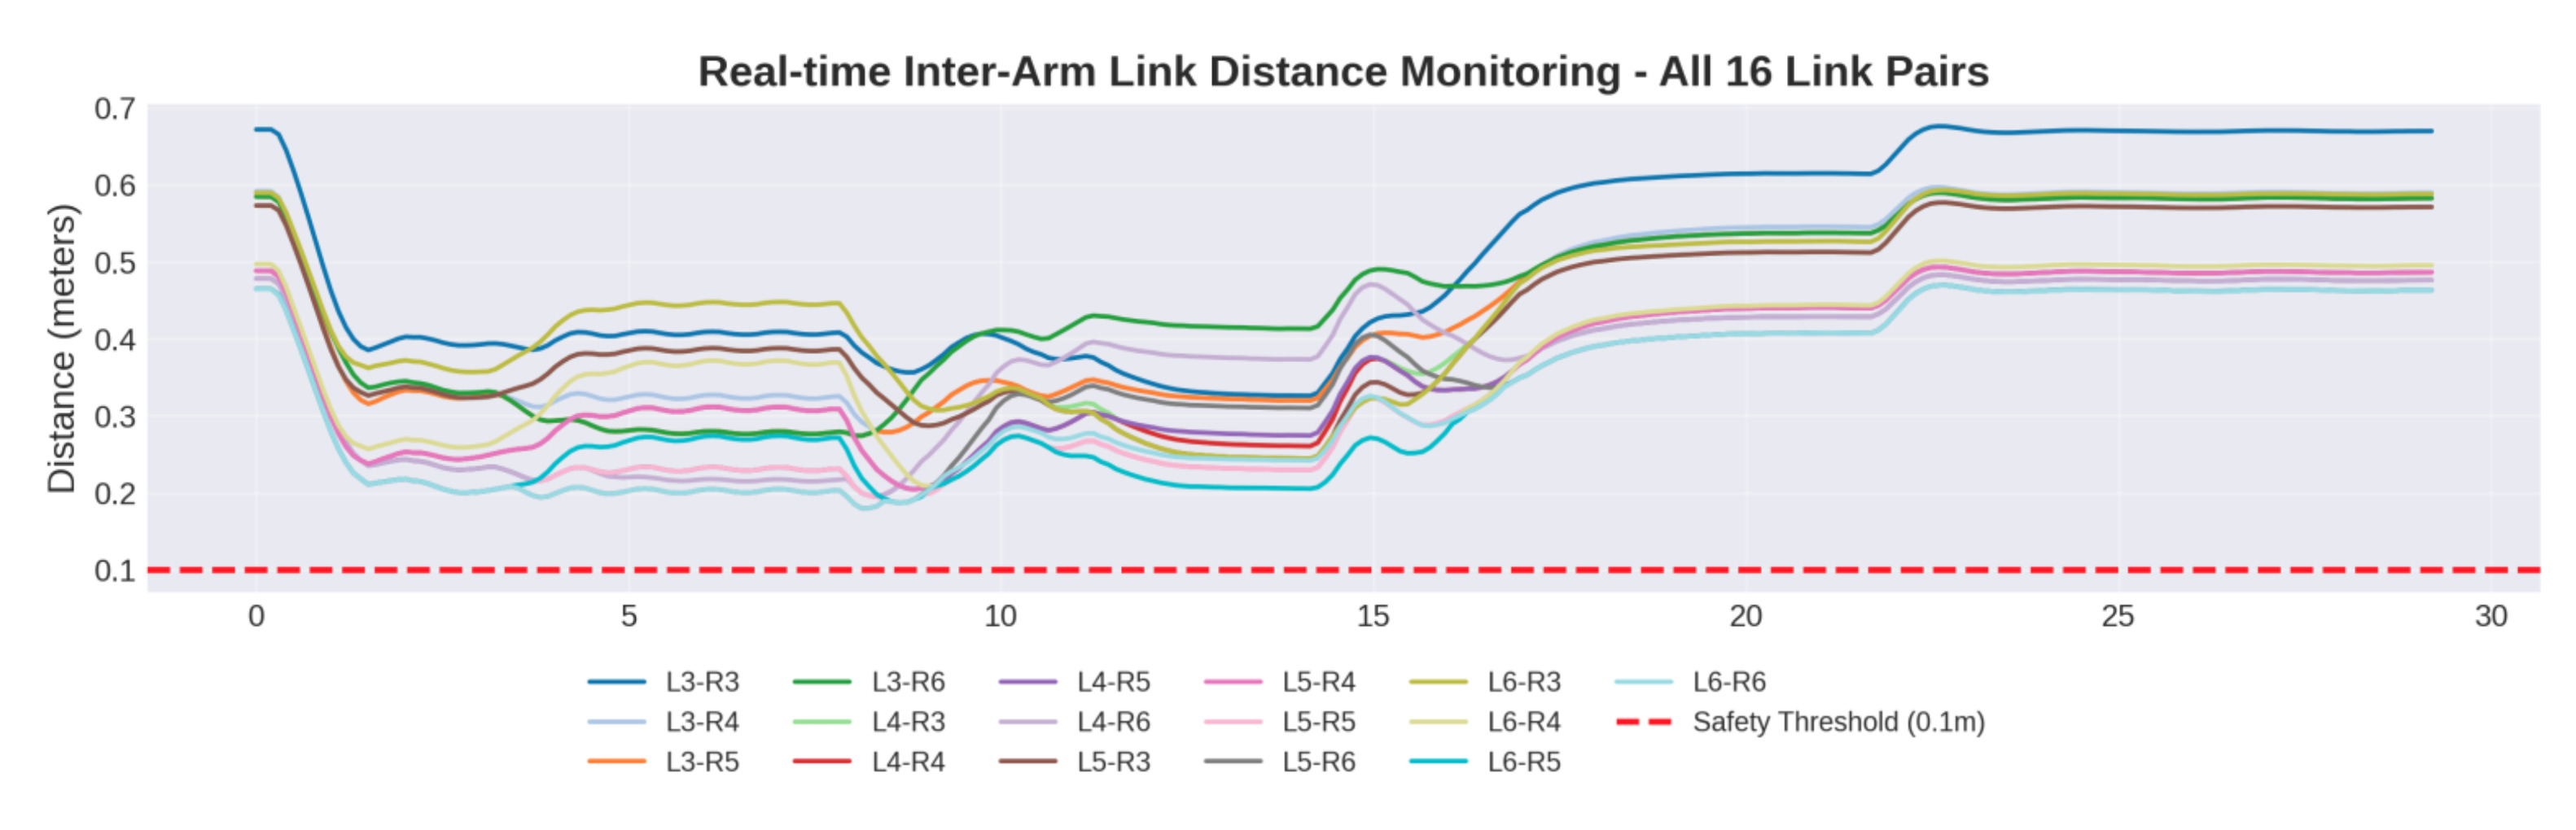
\includegraphics[width=\linewidth]{Images/distanceMonitoring/continuous_distance.jpg}
\caption{Real-time inter-arm link distance monitoring for all sixteen link pairs during the pick
maneuver, against a $0.1$\,m safety threshold~\citep{sk2025distance}.}
\label{fig:dm_continuous}
\end{figure}

Figure~\ref{fig:dm_continuous} shows every monitored pair remaining well clear of the safety
threshold throughout the maneuver, with the closest approach occurring during the pick phase itself
rather than at the start or end, consistent with the arms reaching furthest into the shared
workspace precisely when they are closest to their targets.

\begin{figure}[htbp]
\centering
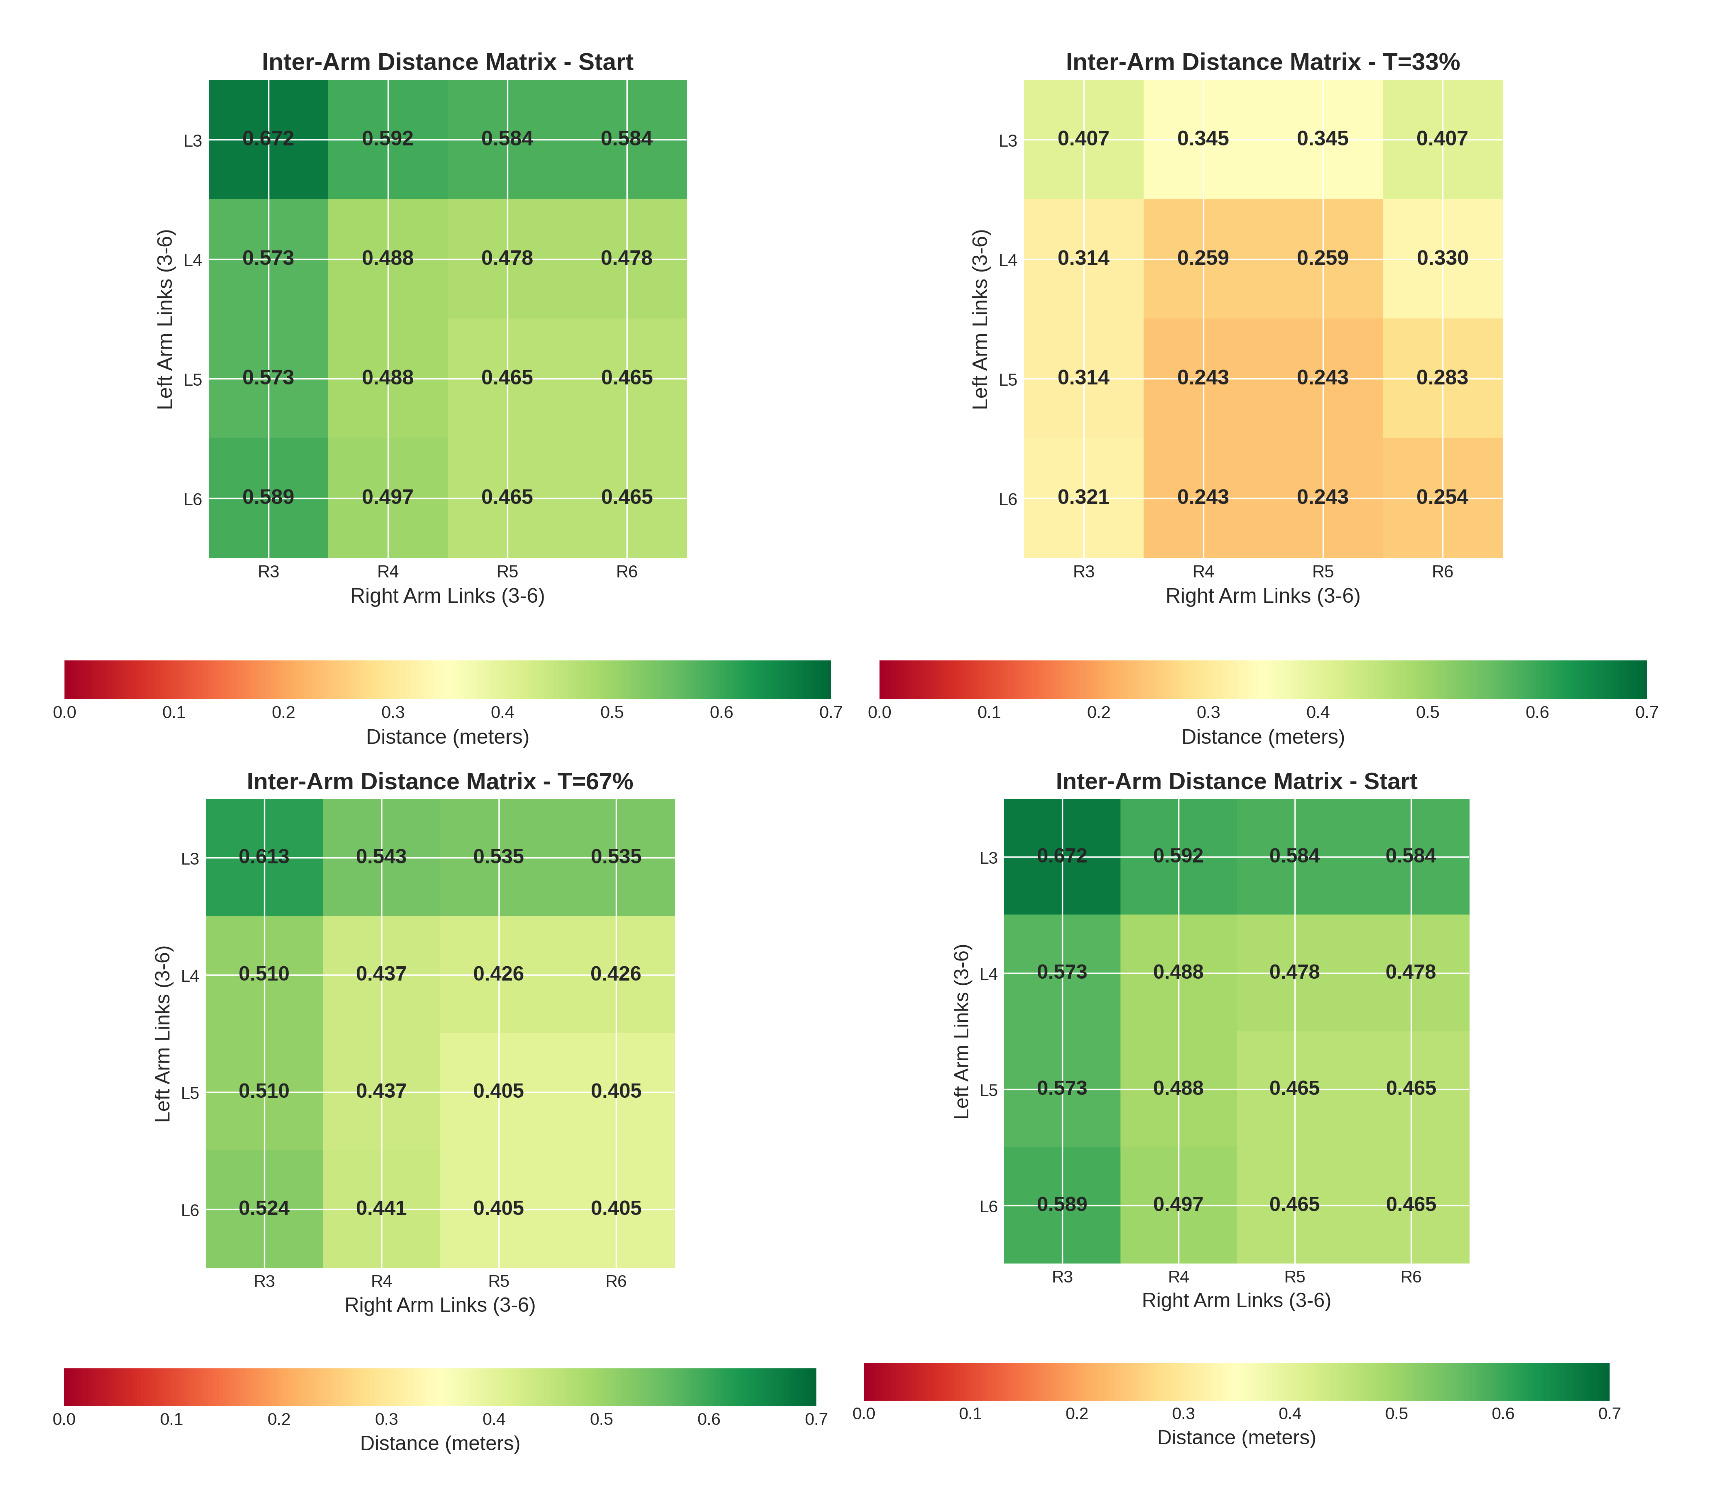
\includegraphics[width=0.75\linewidth]{Images/distanceMonitoring/distance_heatmap.jpg}
\caption{Collision-distance heatmap across four phases: initial separation (start), approach
($T{=}33\%$), closest proximity during the pick operation ($T{=}67\%$), and final separation
(end)~\citep{sk2025distance}.}
\label{fig:dm_heatmap}
\end{figure}

The heatmap in Figure~\ref{fig:dm_heatmap} visualizes the same data across four phases of the
maneuver: initial separation, the approach phase, closest proximity during the pick operation, and
final separation, with darker cells indicating closer link pairs. The closest approaches were
observed between link pairs L4--R4 and L5--R4, dropping to $0.243$\,m and $0.259$\,m respectively at
$T = 33\%$, both comfortably above the $0.1$\,m threshold.

The line-segment kinematic model developed in this chapter provides exactly that: a continuous,
differentiable-in-principle distance signal, computed from joint feedback alone, restricted to the
inter-arm pairs that can actually collide. Chapter 6 builds directly on this signal, coupling the
distance $D_{\text{inter}}$ derived in this chapter to a velocity-aware collision-avoidance
controller, the improved artificial potential field (iAPF) framework that addresses gap G4, for
asymmetric dual-arm motion.
